\documentclass{article}
\usepackage{graphicx}
\usepackage[pdftex]{hyperref}
\begin{document}
\title{Using SLA’s to guide database transition to NoSQL on the cloud: a systematic mapping study}
\author{Fabio Leal $\langle$\href{mailto:sousaleal.fabio@gmail.com}%
{sousaleal.fabio@gmail.com}$\rangle$
\\
Martin A. Musicante $\langle$\href{mailto:mam@dimap.ufrn.br}%
{mam@dimap.ufrn.br}$\rangle$}
\date{\today}
\maketitle  




\begin{abstract}
Cloud computing became a reality over the last years, and many companies are now moving their data-centers to the cloud. 
A concept that is often linked with cloud computing is Infrastructure as a Service (IaaS): the computational infrastructure of a company can now be seen as a monthly cost instead of a number of different factors. 
Recently, a large number of organizations started to replace their relational databases with hybrid solutions (NoSQL DBs, Search Engines, ORDBs). 
These changes are motivated by (\textit{i}) performance improvements on the overall performance of the applications and (\textit{ii}) inability to a RDBMS to provide the same performance of a hybrid solution given a fixed monthly infrastructure cost. 
However, not always the companies can exactly measure beforehand the future impact on the performance on their services by making this sort of technological changes (replace RDBMS by another solution). 
The goal of this systematic mapping study is to investigate the use of Service-Level-Agreements (SLA’s) on database-transitioning scenarios and to verify how SLA’s can be used in this processes.
\end{abstract}

\section{Introduction}

The adoption of cloud-related solutions is growing fast among organizations~\cite{6546068}.
Centralized (mostly mainframe) technology is being replaced by distributed and more flexible forms of data storage and processing.
This change of paradigm is motivated by the necessity to improve the use of resources, as well as by the increasing velocity in which data is produced.

The transition must take into account the quality of the service delivered by the new solutions.
In this context, the notion of Service-Level-Agreements (SLA’s)~\cite{6253526} may be used as a parameter, to guide the process of choosing the most convenient technology.

In this paper, we survey the use of SLA's on database-transitioning scenarios, trying to investigate how they might be used to help the execution this process.
\bigskip

This paper is organized as follows: 
Section~\ref{sec:tts} presents some of the concepts that are related to the transition from a traditional setting to a cloud-aware one.
Section~\ref{sec:asm} presents our research questions and each step of our survey. The outcomes of our Systematic Mapping study can be seen on Section~\ref{sec:outcomes}.

\section{The Technological Shift}
\label{sec:tts}


%\subsection{Cloud Computing}
On the early 90's it was commonplace for every Information Technology (IT) company to have its own Data Center with huge servers and mainframes. 
IT costs were high, and high-performance computing was available only for big companies, as data centers required a lot of physical space and high costs for maintenance~\cite{Armbrust09m.:above}.

The regular way of building a web application was to use client-server approach, where the server was an extremely powerful (and expensive) machine. 
However, new companies, such as Google, were rising with bigger missions: \textit{``to organize the world's information and make it universally accessible and useful''}~\cite{Spector:2012:GHA:2209249.2209262}. 
It was \textit{just} impossible to store the petabytes of daily-generated data in a single server. 

From this point, the community realized that it was much cheaper to build and maintain several low-performance servers than a single high-performance machine.
This approach, however, was incompatible with the traditional way of building applications, as they were designed to work with a single server and database. 

Several research initiatives were conducted in this area and a common solution was rising: to distribute data storage and processing. 
Google, Yahoo and other big IT players helped to build open source tools to make this approach possible, like Hadoop~\cite{5496972}.

This revolution brought to life the notion of \textit{Cloud Computing}, together with new concepts, such as Infrastructure as a Service \textit{(IAAS)}, Platform as a Service \textit{(PAAS)} and Software as a Service \textit{(SAAS)}~\cite{AViewOfCloudComputing}.
The authors in~\cite{AViewOfCloudComputing} say that \textit{Cloud computing refers to both the applications delivered as services over the Internet and the hardware and systems software in the data centers that provide those services.} 


\paragraph*{Data Integration \& Polyglot Persistence}
On the last years, the number of Data Base (DB) Engines grew like never before~\cite{dbranking}. 
Along with the NoSQL movement and expansion of Social Networks, new concepts for Database Models appeared, like Document Store, Search Engines, Key-Value store, Wide Column Store, Multi-Model and Graph DBMS. 
In~\cite{dbranking} a ranking of the most popular DB engines is presented.

Today, instead of having a single Relational Database Management System (DBMS) for the whole application, it is efficient and cost-effective to have several Data Base Engines, one for each type of data that the application handles. 
This concept is called \textit{Polyglot Persistence}~\cite{sadalage2012nosql}.


As \cite{AdressingDataManagementCloud} illustrates, polyglot persistence is very useful in the context of an e-commerce app that deals with a catalog, user access logs, financial information, shopping carts and purchase transactions, for example. The nature of each data type is significantly different (i.e: user logs imply high volume of writes on multiple nodes, shopping carts need high availability and user sessions require rapid access for reads and writes). 

As computing services started to decentralize, developers started to build applications that depended of several data-sources. 
By this time the use of Web Services and Service Oriented Architecture (SOA) became more popular. 


\paragraph*{Service Level Agreements (SLA)}
According to \textit{ITILv3's} official glossary \cite{itilv3glossary}, a Service Level Agreement (SLA) is \textit{an agreement between an IT service provider and a customer. A service level agreement describes the IT service, documents service level targets, and specifies the responsibilities of the IT service provider and the customer.} 

The agreement consists on a set of measurable constraints that a service provider must guarantee to its customers.
In practical terms, it is a document that a service provider delivers to its consumers with minimum quality of service (QoS) metrics. If the service is delivered with a lower QoS than is promised on the SLA, consumers may be refunded or earn benefits that were accorded beforehand.    

\paragraph*{Systematic Mappings}
According to \cite{Petersen:2008:SMS:2227115.2227123}, \textit{"A software engineering systematic map is a defined method to build a classification scheme and structure a software engineering field of interest". 
Systematic Mapping studies provide a global view of a given research field and identify the quantity, results, and the kinds of researches in this field.}

A Systematic map is composed by a number of steps:
\begin{figure}[ht!]
\centering
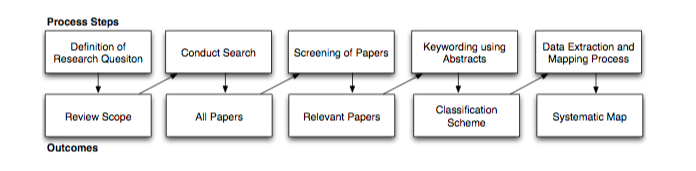
\includegraphics[width=100mm]{pic1.png}
\caption{Systematic Mapping Steps~\cite{Petersen:2008:SMS:2227115.2227123}.\label{fig:sms}}
\end{figure}

On the first step, "Definition of Research question", the questions that must be answered on the survey are defined. On "Review Scope", researchers target the papers/journal sources that will be taken into consideration on the systematic map. After that, the "Search" step is done and "All papers" are retrieved. After a initial "Screening of the papers", the "Relevant papers" are chosen according to inclusion and exclusion criteria defined by the research team. 

Instead of reading the full paper, researchers focus on reading the abstracts and keywords ("Keywording using Abstracts") to classify the papers. After that, a "Classification Scheme" is built. After matching each paper with the classification schema ("Data Extraction and Mapping Process"), the  "Systematic map" is finished. 


\section{A Systematic Mapping}
\label{sec:asm}

In this section we describe how our Systematic Map was coinceived. Some steps of the original process were joined together on this section to simplify the outcomes comprehension.  

\subsection{Definition of the research Scope}
As we want to investigate how SLAs can be used in database transitioning processes, we proposed three research questions to be answered by our study: 

\textbf{RQ1)}  How can SLAs be used to guide database transitioning to NoSQL databases in cloud-based apps? 

\textbf{RQ2)} How can an SLA be used to monitor the performance improvements promised by a database transitioning process?

\textbf{RQ3)} Is there a standard representation of SLAs in cloud services? 

\subsection{Conduct Search for Primary Studies (All Papers)}

We searched for papers on IEEE, ACM and Elsevier, using Google Scholar as a meta-search engine. We also tried to include industry-related conferences, but few of them had online videos available and the vast majority had no written publications.

We used \begin{verbatim}"changes AND database AND nosql AND sla AND cloud"\end{verbatim} as a boolean search string on Google Scholar search engine. This resulted in a total of 88 publications.


\subsection{Screening of papers}
Inclusion and Exclusion criteria were used to filter the list of publications:
\begin{enumerate}
    \item Inclusion Criteria: 
    \begin{itemize}
  		\item English written publications
  		\item Works that make use of SLAs 
    \end{itemize}
    \item Exclusion Criteria
	\begin{itemize}
		\item Access-restriction to the original publication
		\item Non-technical publications 
		\item Publications that don't make any use of SLAs	
    \end{itemize}
    
\end{enumerate}

After applying the inclusion and exclusion criteria our systematic mapping study ended up with 15 relevant publications.

%\newpage
\subsection{Classification of the Papers}

We classified each selected papers in three facets: \textbf{Contribuition}, \textbf{Technology} and \textbf{SLA representation}. On the conceptual map conceptual map we have listed just a subset of the several technology types that were found on the review.

\begin{figure}[!h]
\centering
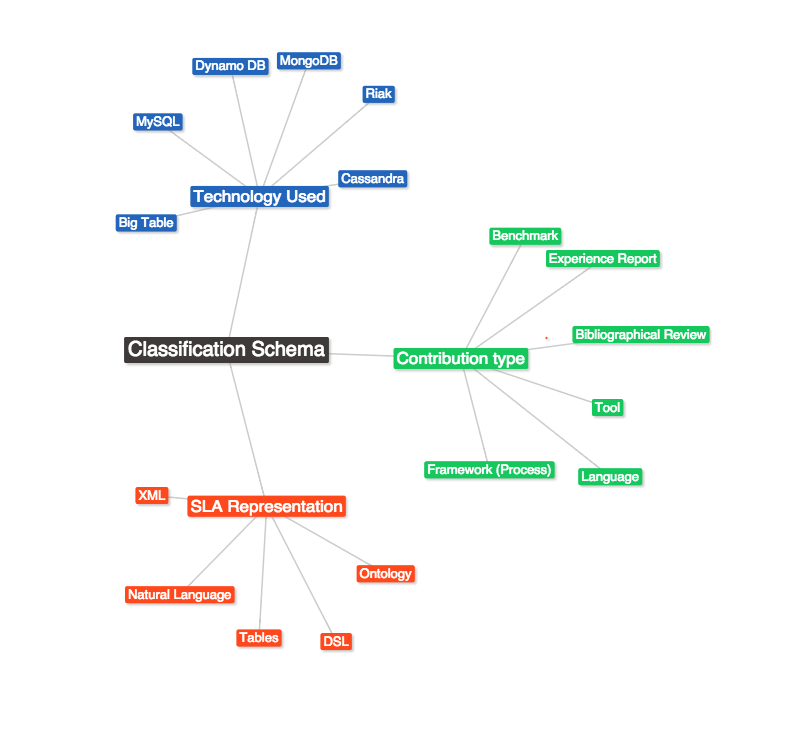
\includegraphics[height=130mm]{pic2.png}
\caption{Classification scheme for selected papers \label{overflow}}
\end{figure}

%\newpage
\section{Outcomes}
\label{sec:outcomes}

As mentioned on "Screening of papers" sub-section, 15 publications were analyzed, and the answers to the research questions are presented below:

\textbf{RQ1)} How can SLAs be used to guide database transitioning to NoSQL databases in cloud-based apps? 

A number of works were found relating SLAs with Quality of Service (QoS) and Quality of Experience (QoE). Several publications, such as \cite{Xiong:2012:DMR:2213598.2213614}, \cite{Konstantinou:2012:TEN:2213836.2213943} and \cite{Klems:2012:RQM:2477172.2477488} propose a SLA-centric approach to monitor and control the performance of cloud-based apps. However, no publication was found addressing the problem of switching from one database technology to another and guiding this process through an SLA. 

\textbf{RQ2)} How can an SLA be used to monitor the performance improvements promised by a database transitioning process?

\cite{6253526}, \cite{6461875}, \cite{6511780} and \cite{Xiong:2011:APA:2038916.2038931} propose SLA-centric/User-Centric solutions to monitor the performance of web applications. All these solutions are technology-agnostic and could be used to monitor the performance improvements promised by a database transitioning process.

\textbf{RQ3)} Is there a standard representation of SLAs in cloud services? 

The selected publications did not present a standardized representation for SLAs. In fact, 60\% of the selected publications did not mention how the SLA was internally represented. 

\cite{6546068} proposes SYBL: \textit{An Extensible Language for Controlling Elasticity in Cloud Applications. SYBL allows specifying in detail elasticity monitoring, constraints, and strategies at different levels of cloud applications, including the whole application, application component, and within application component code. Based on simple SYBL elasticity directives, our runtime system will perform complex elasticity controls for the client, by leveraging underlying cloud monitoring and resource management APIs.}

As a result of the Systematic Map, 5 kinds of representation for SLAs were discovered: DSLs, Relational tales, ontologies and XML variations.


%\newpage
\bibliographystyle{plain}
\bibliography{systematicMapping}	



\end{document}